\documentclass{article}
\usepackage[paperwidth=15cm,paperheight=10cm,margin=0cm]{geometry}
\usepackage[sfdefault]{carlito}
\usepackage[T1]{fontenc}
\usepackage{tikz}
\usetikzlibrary{arrows.meta}
\definecolor{cOurs}{HTML}{4285F4}
\pagestyle{empty}
\begin{document}\noindent
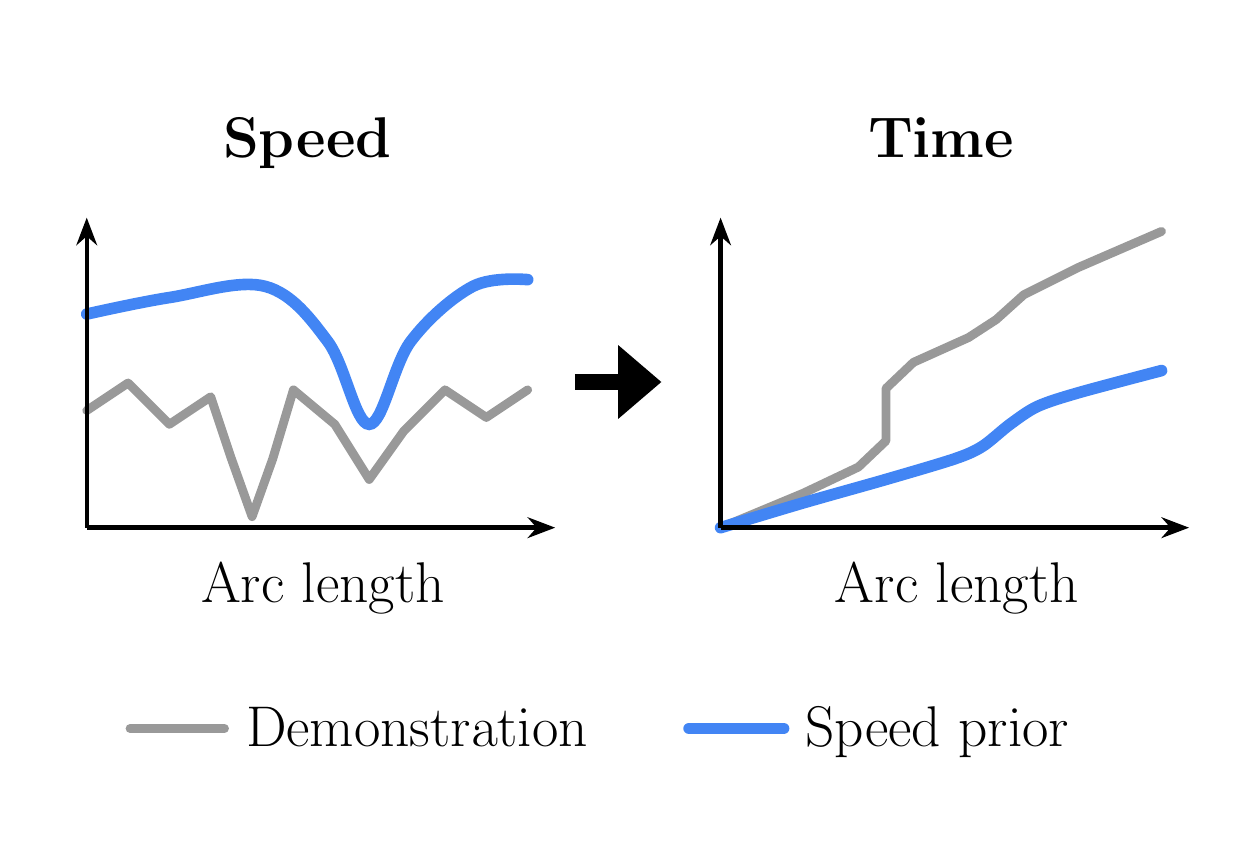
\begin{tikzpicture}[x=1cm,y=1cm,
  lab/.style={font=\fontsize{21}{24}\selectfont},
  ax/.style={-{Stealth[length=3.5mm]}, line width=1.6pt},
  rec/.style={black!40, line width=3.2pt, line join=round, line cap=round},
  ours/.style={cOurs, line width=4.2pt, line cap=round}]
\useasboundingbox (0,0) rectangle (15,10);
% ---- speed
\begin{scope}[shift={(3.55,5.75)}, scale=1.75]
  \draw[rec] (-1.60,-0.35) -- (-1.30,-0.15) -- (-1.00,-0.45) -- (-0.70,-0.25) -- (-0.55,-0.70) -- (-0.40,-1.12) -- (-0.25,-0.70) -- (-0.10,-0.20) -- (0.20,-0.45) -- (0.45,-0.85) -- (0.70,-0.50) -- (1.00,-0.20) -- (1.30,-0.40) -- (1.60,-0.20);
  \draw[ours] plot[smooth, tension=0.6] coordinates {(-1.6,0.35) (-1,0.47) (-0.3,0.55) (0.15,0.15) (0.45,-0.45) (0.75,0.15) (1.2,0.55) (1.6,0.6)};
  \draw[ax] (-1.6,-1.2) -- (1.8,-1.2);
  \draw[ax] (-1.6,-1.2) -- (-1.6,1.05);
\end{scope}
\node[lab, anchor=base, font=\fontsize{21}{24}\bfseries\selectfont] at (3.55,8.35) {Speed};
\node[lab, anchor=base] at (3.75,2.7) {Arc length};
% ---- arrow
\draw[-{Triangle[length=5.5mm, width=9mm]}, line width=6pt] (6.95,5.5) -- (8.05,5.5);
% ---- clock
\begin{scope}[shift={(11.6,5.75)}, scale=1.75]
  \draw[rec] (-1.60,-1.20) -- (-1.00,-0.95) -- (-0.60,-0.76) -- (-0.40,-0.57) -- (-0.40,-0.19) -- (-0.20,0.00) -- (0.20,0.18) -- (0.40,0.31) -- (0.60,0.49) -- (1.00,0.69) -- (1.60,0.95);
  \draw[ours] plot[smooth, tension=0.5] coordinates {(-1.60,-1.20) (-1.00,-1.02) (-0.40,-0.85) (0.10,-0.70) (0.30,-0.61) (0.50,-0.45) (0.70,-0.32) (1.00,-0.22) (1.60,-0.06)};
  \draw[ax] (-1.6,-1.2) -- (1.8,-1.2);
  \draw[ax] (-1.6,-1.2) -- (-1.6,1.05);
\end{scope}
\node[lab, anchor=base, font=\fontsize{21}{24}\bfseries\selectfont] at (11.6,8.35) {Time};
\node[lab, anchor=base] at (11.8,2.7) {Arc length};
% ---- legend
\draw[rec] (1.3,1.1) -- (2.5,1.1); \node[lab, anchor=base west] at (2.65,0.87) {Demonstration};
\draw[ours] (8.4,1.1) -- (9.6,1.1); \node[lab, anchor=base west] at (9.75,0.87) {Speed prior};
\end{tikzpicture}
\end{document}
